\documentclass[10pt]{beamer}

% Theme selection
\usetheme{metropolis} % Clean, modern, "research-style" theme
\usecolortheme{owl}     % Dark theme (premium feel) or use standard for white
% \usecolortheme{beaver} % For professional red/white theme

% Packages
\usepackage{graphicx}
\usepackage{booktabs}
\usepackage{hyperref}
\usepackage{tikz}
\usetikzlibrary{shapes,arrows,positioning}

% Title page details
\title{InternDesk}
\subtitle{A Full-Stack Intern Management Platform}
\author{Research and Development Team}
\date{\today}
\institute{Advanced Software Engineering Lab}

\begin{document}

% Slide 1: Title
\begin{frame}
    \titlepage
\end{frame}

% Slide 2: Project Overview
\begin{frame}{Project Overview}
    \textbf{InternDesk} is a comprehensive management ecosystem designed to streamline the lifecycle of internships. 
    \vspace{0.5cm}
    \begin{itemize}
        \item Centralized platform for Interns, Mentors, and Managers.
        \item Real-time tracking of tasks and milestones.
        \item Integrated communication and feedback loops.
    \end{itemize}
\end{frame}

% Slide 3: Problem Statement
\begin{frame}{1. Problem Statement}
    Traditional internship management faces several challenges:
    \vspace{0.5cm}
    \begin{enumerate}
        \item \textbf{Fragmentation:} Communication over email, tasks on spreadsheets, and feedback in documents.
        \item \textbf{Visibility Gap:} Managers often lack a high-level view of all intern progress.
        \item \textbf{Role Ambiguity:} Difficulty in distinguishing responsibilities between Mentors and Managers.
        \item \textbf{Scalability:} Manual tracking becomes impossible as the number of interns grows.
    \end{enumerate}
\end{frame}

% Slide 4: Proposed Solution
\begin{frame}{2. Working Solution}
    InternDesk solves these issues by providing dedicated interfaces for each stakeholder:
    \vspace{0.3cm}
    \begin{itemize}
        \item \textbf{Intern Dashboard:} View tasks, submit progress, and communicate with mentors.
        \item \textbf{Mentor Portal:} Assign tasks, provide feedback, and monitor specific intern groups.
        \item \textbf{Manager View:} Oversee the entire program, manage user roles, and analyze program performance.
    \end{itemize}
    \vspace{0.3cm}
    \textit{Features include role-based access control (RBAC), real-time notifications, and persistent data storage.}
\end{frame}

% Slide 5: Tech Stack
\begin{frame}{3. Tech Stack}
    Built with a modern, scalable, and type-safe stack:
    \vspace{0.5cm}
    \begin{columns}[T]
        \begin{column}{0.48\textwidth}
            \textbf{Frontend}
            \begin{itemize}
                \item React 18
                \item TypeScript
                \item Vite (Build Tool)
                \item Pure CSS (Modular)
            \end{itemize}
        \end{column}
        \begin{column}{0.48\textwidth}
            \textbf{Backend \& DB}
            \begin{itemize}
                \item Node.js
                \item Express.js
                \item PostgreSQL
                \item JWT Authentication
            \end{itemize}
        \end{column}
    \end{columns}
\end{frame}

% Slide 6: System Architecture
\begin{frame}{System Architecture}
    \begin{center}
    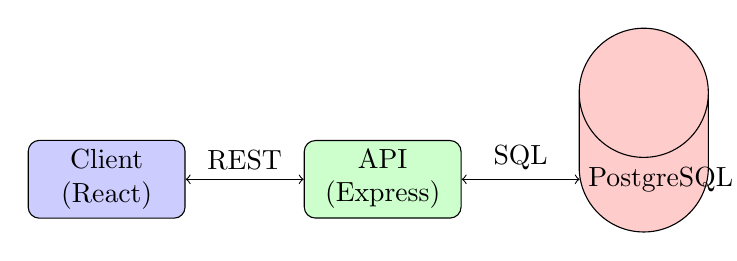
\begin{tikzpicture}[node distance=1.5cm, auto]
        \node [rectangle, draw, fill=blue!20, text width=5em, text centered, rounded corners, minimum height=2em] (client) {Client (React)};
        \node [rectangle, draw, fill=green!20, text width=5em, text centered, rounded corners, minimum height=2em, right=of client] (api) {API (Express)};
        \node [cylinder, draw, fill=red!20, text width=4em, text centered, minimum height=3em, shape border rotate=90, right=of api] (db) {PostgreSQL};
        
        \draw [<->] (client) -- (api) node[midway, above] {REST};
        \draw [<->] (api) -- (db) node[midway, above] {SQL};
    \end{tikzpicture}
    \end{center}
    \vspace{0.5cm}
    \begin{itemize}
        \item Decoupled Frontend and Backend for scalability.
        \item Secure API endpoints protected by Middleware.
        \item ACID-compliant database for data integrity.
    \end{itemize}
\end{frame}

% Slide 7: Key Features
\begin{frame}{Key Features}
    \begin{description}
        \item[Task Management] Dynamic task assignment and status tracking.
        \item[Real-time Feedback] Instant notifications and review systems.
        \item[Role Persistence] Context-aware navigation and session management.
        \item[Responsive Design] Optimized for desktops and mobile devices (sidebar toggle).
        \item[Production Ready] Scalable deployment configurations (Managed PostgreSQL).
    \end{description}
\end{frame}

% Slide 8: Future Work
\begin{frame}{Conclusion \& Future Work}
    \textbf{Current Status:} Fully functional prototype with core management features.
    \vspace{0.5cm}
    \textbf{Future Enhancements:}
    \begin{itemize}
        \item AI-driven intern performance analytics.
        \item Video conferencing integration for mentor-intern syncs.
        \item Automated certificate generation upon completion.
    \end{itemize}
\end{frame}

% Slide 9: Contact
\begin{frame}{Questions?}
    \begin{center}
        \Huge Thank You!
        \vspace{1cm}
        \large
        \textbf{Project Repository:} \url{https://github.com/your-repo/interndesk} \\
        \textbf{Contact:} research@interndesk.com
    \end{center}
\end{frame}

\end{document}
